\documentclass[11pt,letterpaper]{article}
\usepackage[margin=0.85in]{geometry}
\usepackage[T1]{fontenc}
\usepackage{lmodern}
\usepackage{microtype}
\usepackage{amsmath,booktabs,longtable,array}
\usepackage{pgfplots}
\usetikzlibrary{arrows.meta,patterns,positioning}
\usepgfplotslibrary{groupplots}
\pgfplotsset{compat=1.18}
\usepackage[hidelinks]{hyperref}
% The export script supplies this digest to bind a PDF to its exact source.
\ifdefined\ManuscriptSourceSHA
\hypersetup{pdfsubject={Manuscript source SHA256: \ManuscriptSourceSHA}}
\fi
\usepackage{caption}
\captionsetup{font=small,labelfont=bf}
\setlength{\parindent}{0pt}
\setlength{\parskip}{0.45em}
\setlength{\emergencystretch}{2em}
\renewcommand{\arraystretch}{1.16}
\title{Fit Quality Screening of Biochar\texorpdfstring{\\}{ }for Phosphorus Capture}
\author{}
\date{Research note for scientific discussion\\5 October 2026}
\begin{document}
\maketitle
\vspace{-1.8em}
\begin{center}\small A reproducible secondary analysis using GIGI\end{center}

\begin{abstract}
Selecting biochars for phosphorus capture requires distinguishing a large fitted capacity from a well-supported estimate and from measured performance in runoff. This note reanalyzes 36 published formulation-level Langmuir summaries from a poultry-litter biochar experiment. Capacity estimates, reported standard errors, fit quality and net-release labels were retained in a queryable GIGI dataset. Applying the descriptive screen $R^2>0.80$ retained 16 formulations, excluded eight numeric fits and preserved 12 net-release entries without assigning them zero capacity. All nine formulations prepared using 1~M magnesium activation passed this screen; none of the nine untreated formulations did. The largest retained point estimate was $10.35\pm1.45$~mg~P/g biochar, whereas the largest unscreened estimate was $134.41\pm133.98$~mg~P/g with $R^2=0.00$. Here, $\pm$ denotes the source-reported standard error. Tightening the screen to $R^2>0.90$ changed the highest-ranked formulation. The resulting shortlist is therefore conditional on model screening and does not identify a statistically established optimum. The contribution is a transparent and verified data workflow, not new sorption experiments or proof of reduced field runoff. A proposed follow-up protocol links material screening to P mass balances, breakthrough and release testing.
The archived workbook additionally contributes 540 measured isotherm pairs, including 171 negative sorption values; all were preserved and independently checked after import. These observations support descriptive release screening but do not constitute independent field trials.
\end{abstract}

\section{Research question and scope}
The practical question is which biochar formulations warrant additional testing for phosphorus capture. An appropriate workflow must retain evidence of weak fits and phosphorus release, rather than report only a ranked list of capacities. It must also preserve the distinction between a model parameter and a directly measured environmental outcome.

The sources are Table~1 of Padilla et al.~\cite{padilla} and the accompanying Dryad isotherm worksheet~\cite{dryad}, covering three poultry-litter feedstock age categories, four magnesium activation concentrations and three pyrolysis temperatures. Each of the 36 rows in the expanded table represents a formulation-level summary, not an independent experimental replicate. A separate dataset preserves 540 measured concentration--sorption pairs. The present note analyzes both layers descriptively. It does not reproduce the authors' inferential analysis or claim new evidence for a sorption mechanism.

Three questions are addressed: which reported capacity estimates survive a declared fit-quality screen; how sensitive the shortlist is to that screen; and how GIGI can preserve and query the evidence needed for a subsequent laboratory program. Crop-uptake outcomes from the earlier exploratory work are outside this note because they do not measure P removal from water.

\section{What a fiber bundle database means}
\subsection{A sample tray with a measurement card at every position}
Imagine a laboratory sample tray. Each occupied position has a permanent label, such as formulation~24. Above that position is a measurement card with spaces for the recipe, capacity estimate, standard error, fit quality and source reference. The tray's labeled positions answer \emph{which formulation?}; the card answers \emph{what is recorded about it?}

In the fiber-bundle analogy, the labeled positions form the \textbf{base space}. The collection of possible measurements and attributes attached to one position is its \textbf{fiber}. The collection of positions together with their attached fibers is the \textbf{bundle}. A stored record supplies the actual values on a card. Using the same card layout across the tray makes it possible to retrieve, filter and compare records consistently.

The distinction between possible and observed values matters. A blank capacity box still exists on an NR record's card; it has not become a measurement of zero. Similarly, a formulation's unique label identifies its record but does not tell us how chemically similar it is to another formulation. Formulation~24 is not physically ``closer'' to formulation~25 merely because their identifiers are consecutive.

\begin{center}
\begin{tabular}{@{}p{0.25\textwidth}p{0.65\textwidth}@{}}
\toprule
Analogy & This dataset\\\midrule
Labeled tray position & Base key: formulation ID 24\\
Measurement card & Fiber fields: PL3, 1~M Mg, 900~$^\circ$C, capacity, SE, $R^2$, provenance\\
Completed card & Observed values: $10.35$, $1.45$ and $0.90$, with units and field meanings\\
Whole tray & The named bundle containing all 36 formulation records\\
\bottomrule
\end{tabular}
\end{center}

\subsection{Where geometry enters and what the analogy leaves out}
\begin{figure}[htbp]
\centering
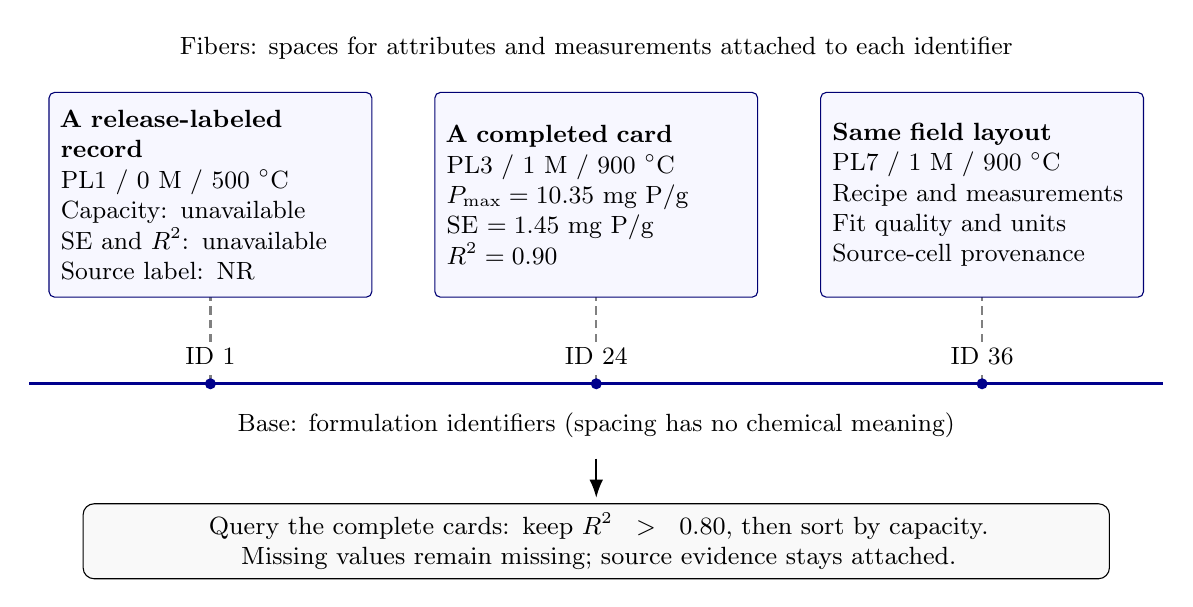
\begin{tikzpicture}[x=1cm,y=1cm,>=Latex,font=\small]
\draw[very thick,blue!55!black] (0,0) -- (14.4,0);
\node[anchor=north] at (7.2,-0.25) {Base: formulation identifiers (spacing has no chemical meaning)};
\foreach \x/\id in {2.3/1,7.2/24,12.1/36}{
 \draw[densely dashed,gray,thick] (\x,0) -- (\x,1.1);
 \fill[blue!55!black] (\x,0) circle (2pt);
 \node[fill=white,inner sep=2pt] at (\x,0.35) {ID \id};
 \draw[rounded corners=2pt,fill=blue!3,draw=blue!45!black] (\x-2.05,1.1) rectangle (\x+2.05,3.7);
}
\node[align=left,text width=3.8cm] at (2.3,2.4) {\textbf{A release-labeled record}\\PL1 / 0 M / 500 $^\circ$C\\Capacity: unavailable\\SE and $R^2$: unavailable\\Source label: NR};
\node[align=left,text width=3.8cm] at (7.2,2.4) {\textbf{A completed card}\\PL3 / 1 M / 900 $^\circ$C\\$P_{\max}=10.35$ mg P/g\\SE $=1.45$ mg P/g\\$R^2=0.90$};
\node[align=left,text width=3.8cm] at (12.1,2.4) {\textbf{Same field layout}\\PL7 / 1 M / 900 $^\circ$C\\Recipe and measurements\\Fit quality and units\\Source-cell provenance};
\node[anchor=south] at (7.2,4.0) {Fibers: spaces for attributes and measurements attached to each identifier};
\draw[->,thick] (7.2,-0.95) -- (7.2,-1.45);
\node[draw,rounded corners,align=center,fill=gray!5,text width=12.8cm] at (7.2,-2.0)
 {Query the complete cards: keep $R^2>0.80$, then sort by capacity.\\Missing values remain missing; source evidence stays attached.};
\end{tikzpicture}
\caption{Conceptual drawing of the fiber-bundle organization used here. Three records illustrate the base--fiber distinction; the full bundle contains 36. The connecting lines show attachment, not causal relationships or a measured geometric distance.}
\label{fig:bundle}
\end{figure}

A fiber bundle is a mathematical way to organize local spaces over a base. In geometry, a section selects a value in the fiber over each base point. For this finite database, the stored records can be understood as a discrete assignment of values to indexed positions. This explanation provides intuition; the sample tray is not a claim that the experimental design has been shown to form a smooth physical manifold.

GIGI uses this organization as a basis for database operations and geometric analyses~\cite{gigi}. For example, a collection of numeric measurement cards can be studied for neighborhood structure or unusual records when the selected representation and distance rule are appropriate. Those comparisons require scientific choices: units, scaling, categorical encoding, missingness and which fields should enter a distance. A difference of one in temperature, capacity and $R^2$ does not carry the same meaning. The database cannot make that experimental judgment merely from a field name.

In this note, the base key is the unique formulation identifier; recipe, measurement and provenance fields live with that key. We use GIGI to preserve complete cards and to ask an explicit question: retain records whose reported $R^2$ exceeds the chosen threshold, then rank their capacities. Conventional databases or analysis scripts can perform the same screening. No advantage of geometric learning is inferred here, and GIGI's geometric metadata are not substitutes for the experiment's SE, model diagnostic or runoff validation.

\section{Data and analytical methods}
\subsection{Source and measurement context}
Published capacity estimates, standard errors (SE), $R^2$ values and NR labels were extracted with source-cell identifiers. The table defines NR as net P release. These entries were stored as null capacity, SE and $R^2$, not as zero. Feedstock codes PL1, PL3 and PL7 identify litter aged 1, 3--5 and 7--9 years, respectively. Magnesium activation concentration refers to the preparation solution, not the final Mg content of the biochar.

The source batch tests used 0.1~g biochar in 20~mL solution, initial P of 25--150~mg/L, 10~mM KCl, initial pH around 5 and 24~h equilibration at 21~$^\circ$C; experiments were conducted in triplicate~\cite{padilla}. These conditions constrain transfer to runoff water. After an initial direct-download failure, the public Dryad workbook~\cite{dryad} was supplied as the 10 October 2023 archive. Its unchanged bytes and README are preserved with SHA-256 digests. The worksheet \texttt{Figure 5 and Sup. Fig. S5} supplies 540 paired solution-concentration and sorbed-P values: 15 points for each of the 36 formulations. These measured pairs are analyzed descriptively in addition to the published fit summaries; they are not used here to refit the Langmuir parameters.

Each pair retains its sheet name and Excel cell coordinates. Point indices preserve sheet order; no experimental-unit identity, initial concentration, or replicate assignment is inferred solely from position. Negative sorbed-P values are retained as net release. The 540 rows pool multiple concentration conditions and within-condition measurements and must not be treated as 540 independent manufacturing batches. The workbook's notes refer to a nonexistent \texttt{Figure 4 and Sup. Fig. S5} tab; the actual isotherm tab was identified by its headers. Two other sheets use PL9 labels where the paper's age category is PL7. Those sheets are archived but not merged into the isotherm analysis or silently relabeled.

\subsection{Descriptive screening and ranking}
For a formulation $i$, inclusion in the primary numerical shortlist was defined as
\begin{equation}
I_i=\mathbf{1}\{P_{\max,i}\text{ is reported and }R_i^2>0.80\}.
\label{eq:screen}
\end{equation}
This follows the threshold in the source figure description. The article also describes excluding $R^2<0.80$ elsewhere. No displayed value equals 0.80, so that wording difference does not change the primary result. All thresholds in this analysis are explicitly strict and operate on the published values rounded to two decimal places.

Retained records were ordered by decreasing $P_{\max}$. Group counts use all nine formulations at each Mg concentration as their denominator. Capacity ranges describe only the retained subset. No imputation, inverse-variance pooling, new hypothesis test, confidence interval, or causal comparison between Mg levels was performed. The source-reported SE was carried with each estimate rather than converted into a nominal 95\% interval without the necessary fit details.

Sensitivity analyses repeated the rule with $R^2>0.70$, $>0.85$, $>0.90$ and $>0.95$. These are alternative descriptive screens, not independently calibrated standards for sorbent suitability. A good $R^2$ does not establish correct model specification, an unbiased parameter estimate, independent predictive accuracy, or field performance.

\subsection{Implementation and verification}
Python's standard library extracted the attributed HTML table excerpt into JSON and CSV and computed an independent reference result. GIGI stored the formulation records and executed filtering, ranking and grouped aggregation. A complete roundtrip checked identifiers, text and nulls exactly and numeric fields within $10^{-12}$ relative or absolute tolerance. Returned rankings at all five thresholds and the grouped counts and means were compared with the independent reference.

A synthetic check planted a capacity of 9999 with $R^2=0.01$ and a capacity of 5 with $R^2=0.95$. The screened query had to select the latter. Removing the fit condition had to select the former, demonstrating that the verification distinguishes the screening mechanism from capacity-only ranking. Synthetic records occupy a separate bundle. The repository includes deterministic offline tests and exact live HTTP receipts.

GIGI's geometric confidence metadata were not used as statistical uncertainty. No spectral clustering, manifold prediction or performance comparison against conventional statistical software was undertaken. The demonstrated contribution is reproducible evidence handling with the measurements and their qualifications co-located.

\section{Results}
\subsection{Primary screen}
Of the 36 formulations, 24 had numeric capacity estimates and 12 carried NR labels. Sixteen numeric estimates satisfied Equation~\ref{eq:screen}; eight did not. Table~\ref{tab:activation} shows that the 1~M group contains nine retained estimates, while the untreated group contains seven NR entries and two excluded numeric fits. This does not mean that all untreated materials have exactly zero uptake under every condition. The table does not quantify their release, and an excluded model may summarize a condition-dependent response poorly.

\begin{table}[htbp]
\centering\small
\caption{Primary screening outcomes by activation concentration. Ranges summarize retained estimates only and are not uncertainty intervals. Each formulation is counted once.}
\label{tab:activation}
\begin{tabular}{@{}rrrrrl@{}}
\toprule
Mg (M) & Total & Retained & Excluded & NR & Range (mg P/g)\\
\midrule
@@ACTIVATION_ROWS@@
\bottomrule
\end{tabular}
\end{table}

The highest retained point estimate was PL3 at 1~M Mg and 900~$^\circ$C: $10.35\pm1.45$~mg~P/g, with $R^2=0.90$. In comparison, PL1 at 1~M and 500~$^\circ$C was $8.55\pm0.97$~mg~P/g, with $R^2=0.94$. Figure~\ref{fig:capacity} displays all retained estimates with their reported SE. Neither the ordering of point estimates nor visual overlap of SE bars is a formal pairwise test. Unknown dependence between fitted estimates prevents treating these bars as independent experimental-batch uncertainty.

The unscreened maximum, PL7 at 0.5~M and 500~$^\circ$C, was $134.41\pm133.98$~mg~P/g with $R^2=0.00$. Its SE is approximately as large as the estimate itself. The screening workflow excludes this value from the numerical shortlist but keeps it in the source inventory. This illustrates a failure of capacity-only ranking without implying that a fit threshold alone validates the remaining models.

\begin{figure}[p]
\centering
\begin{tikzpicture}
\begin{axis}[
 width=0.89\textwidth,height=0.62\textheight,
 xmin=0,xmax=13,ymin=0.4,ymax=16.6,
 xlabel={Published $P_{\max}$ (mg P/g biochar)},
 ytick={1,...,16},yticklabels={@@PLOT_LABELS@@},
 yticklabel style={font=\small},xticklabel style={font=\small},
 grid=major,grid style={gray!18},axis line style={gray!60},
 tick style={gray!60},
 title={Feedstock / Mg activation (M) / pyrolysis temperature ($^\circ$C)},
 title style={font=\small},
]
\addplot+[only marks,mark=*,mark size=2.4pt,color=blue!55!black,
 error bars/.cd,x dir=both,x explicit]
 table[x index=0,y index=1,x error index=2,header=false]{
@@PLOT_DATA@@
};
\end{axis}
\end{tikzpicture}
\caption{All 16 estimates retained at $R^2>0.80$, ranked by point estimate. Horizontal bars are the \emph{published standard errors}, not 95\% confidence intervals and not field-performance ranges. Values are replotted from Table~1 of Padilla et al.~\cite{padilla}. The leading estimate is not a statistically established winner.}
\label{fig:capacity}
\end{figure}

\subsection{Threshold sensitivity}
Tightening the strict threshold changes both the set of retained formulations and the largest retained point estimate (Table~\ref{tab:sensitivity}). At $R^2>0.90$, the PL3/1~M/900~$^\circ$C formulation is excluded because its displayed $R^2$ equals 0.90. PL1/1~M/500~$^\circ$C becomes the highest-ranked retained formulation. At $R^2>0.95$, PL1/1~M/700~$^\circ$C leads. These changes show that a unique recipe recommendation would depend on an analyst-selected cutoff and on the precision of the published fit diagnostic.

The concentration-level result is more stable across the first three thresholds: all nine 1~M formulations remain eligible at 0.70, 0.80 and 0.85. Seven remain at 0.90 and four at 0.95. This supports prioritizing multiple 1~M formulations for further comparison within this dataset, while retaining lower-activation candidates when testing chemical-use and performance tradeoffs. Costs and manufacturing energy were not measured here.

\begin{table}[htbp]
\centering\small
\caption{Sensitivity to a strict $R^2$ cutoff. Every leading recipe uses 1~M Mg. Capacities are point estimates $\pm$ published SE. Equality with the cutoff is excluded.}
\label{tab:sensitivity}
\begin{tabular}{@{}rrrll@{}}
\toprule
Cutoff & Retained & At 1 M & Leading feedstock, $^\circ$C & Capacity (mg P/g)\\
\midrule
@@SENSITIVITY_ROWS@@
\bottomrule
\end{tabular}
\end{table}

\subsection{Descriptive analysis of the underlying isotherm measurements}
The supplied workbook contains 540 paired observations across the same 36 formulations. Of these, 171 have negative sorbed-P values. Grouped descriptively by activation concentration, the counts are 93/135 at 0~M, 52/135 at 0.25~M, 26/135 at 0.5~M and 0/135 at 1~M. Every recorded 1~M point in this sheet is positive, ranging from 1.47 to 13.47~mg~P/g. These denominators count observations over different concentrations and materials, not independent studies. They do not estimate the probability of success in runoff or establish a causal dose response.

Figure~\ref{fig:raw} preserves the signed measurements and their solution-concentration coordinates. A formulation can show uptake at some conditions and release at others, so the sign of an individual observation and a formulation-level NR label answer different questions. The numerical values were loaded into a separate GIGI bundle, fully checked against the source-derived reference, and queried for negative sorption; all 171 returned records matched. No summary fit was replaced by an ad hoc fit to these points.

\begin{figure}[p]
\centering
\begin{tikzpicture}
\begin{groupplot}[group style={group size=2 by 2,horizontal sep=1.7cm,vertical sep=2.1cm},
 width=0.40\textwidth,height=0.30\textheight,
 xmin=0,xmax=190,ymin=-13,ymax=23,
 xlabel={Solution P (mg/L)},ylabel={Sorbed P (mg/g)},
 ticklabel style={font=\small},label style={font=\small},title style={font=\small},
 grid=major,grid style={gray!15},]
@@RAW_PLOTS@@
\end{groupplot}
\end{tikzpicture}
\caption{All 540 archived isotherm observations, separated by Mg activation concentration, with common axes. Points pool three feedstocks and three temperatures within each panel (135 points). Negative values indicate net release; the dashed line denotes zero. No curve fitting, smoothing, inferred replicate identities, or independence assumption is used. Coincident points may overlap. Source: Dryad isotherm worksheet~\cite{dryad}.}
\label{fig:raw}
\end{figure}

\section{Interpretation and limitations}
\subsection{Saturation capacity is not removal at a target concentration}
A fitted maximum does not determine uptake at a specific water concentration. In the Langmuir form,
\begin{equation}
q(C_e)=\frac{P_{\max}K C_e}{1+K C_e},
\end{equation}
the affinity parameter $K$ is required along with $P_{\max}$. The analyzed table does not supply $K$. Consequently, it cannot support predicting effluent quality or sizing a treatment unit for a specified dilute influent. Extrapolation from 24-hour batch tests to short-contact runoff treatment also requires kinetic and transport evidence. Fitting a linearized isotherm changes the error structure relative to fitting the original concentration-response relationship; residual diagnostics and alternative fits cannot be checked from these summaries.

\subsection{Sampling and uncertainty}
These 36 formulations belong to one experiment and do not represent 36 independent studies or manufacturing batches. Feedstock age labels are also material identities; they do not isolate an age effect from all other feedstock differences. Source-reported parameter SE does not quantify scale-up variation, seasonal water chemistry, aging, or field-to-field variation. No claim of a general optimum, a causal Mg dose response, or a reduction in agricultural P export follows from this analysis.

Conditioning on a fit screen changes the composition of each activation subset. Comparing retained means without accounting for that selection could overstate a material advantage. NR and excluded fits therefore remain visible in the denominators and full inventory. Low $R^2$ can identify an unreliable capacity estimate without identifying the physical reason for the poor fit.

\subsection{Source fidelity}
The table reports PL7/0.25~M/900~$^\circ$C as $0.62\pm0.06$~mg~P/g with $R^2=0.96$, whereas the article narrative reports a minimum of 0.66~mg~P/g. The tabulated value was retained without correction and is flagged for author or model-reconstruction verification. All 36 formulation summaries are provided in Appendix~\ref{app:inventory}. Access to the workbook resolves the earlier download limitation, but descriptive extraction alone does not resolve this table/text discrepancy or reproduce the original model fitting. Formal comparisons require a reviewed error model and experimental-unit mapping.

\section{A proposed validation study for runoff applications}
The next experiment should ask whether candidate materials remove P from the target water at realistic contact times and retain it through subsequent exposure. This is a proposed protocol, not an experiment performed in the present work.

\begin{figure}[htbp]
\centering
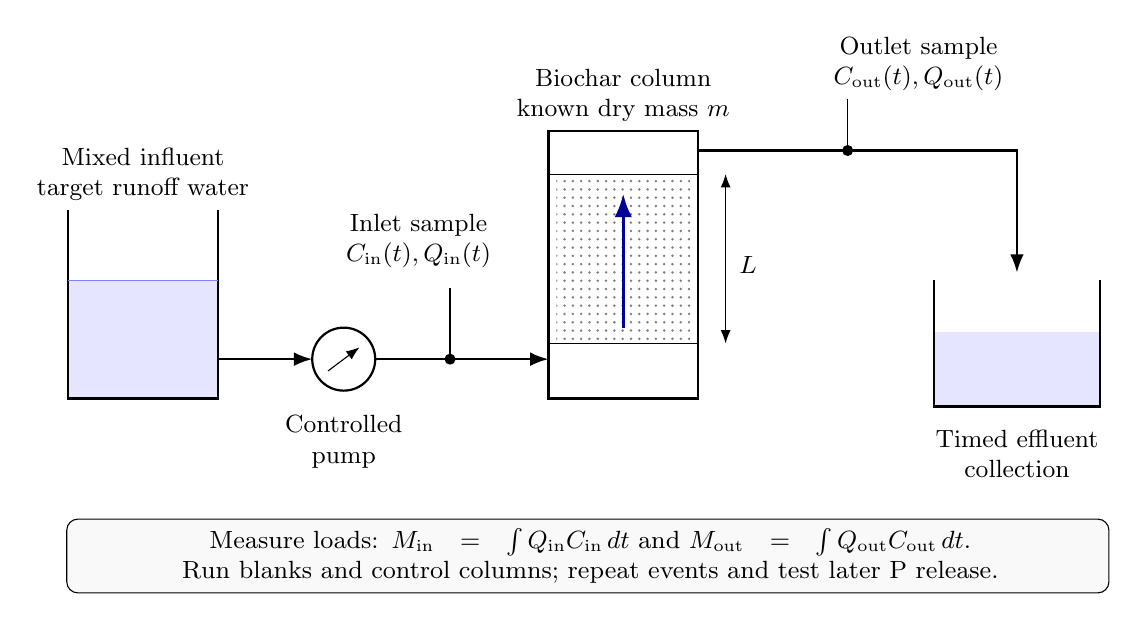
\begin{tikzpicture}[x=1cm,y=1cm,>=Latex,font=\small]
\fill[blue!10] (0.2,0.8) rectangle (2.1,2.3);
\draw[thick] (0.2,3.2) -- (0.2,0.8) -- (2.1,0.8) -- (2.1,3.2);
\draw[blue!50] (0.2,2.3) -- (2.1,2.3);
\node[align=center] at (1.15,3.65) {Mixed influent\\target runoff water};
\draw[->,thick] (2.1,1.3) -- (3.3,1.3);
\draw[thick] (3.7,1.3) circle (0.4);
\draw[->] (3.5,1.15) -- (3.9,1.45);
\node[align=center] at (3.7,0.25) {Controlled\\pump};
\draw[->,thick] (4.1,1.3) -- (6.3,1.3);
\draw[thick] (6.3,0.8) rectangle (8.2,4.2);
\fill[pattern=dots,pattern color=black!50] (6.4,1.5) rectangle (8.1,3.65);
\draw (6.3,1.5) -- (8.2,1.5) (6.3,3.65) -- (8.2,3.65);
\draw[->,very thick,blue!60!black] (7.25,1.7) -- (7.25,3.4);
\node[align=center] at (7.25,4.65) {Biochar column\\known dry mass $m$};
\draw[<->] (8.55,1.5) -- (8.55,3.65);
\node[anchor=west] at (8.6,2.5) {$L$};
\draw[->,thick] (8.2,3.95) -- (12.25,3.95) -- (12.25,2.4);
\fill[blue!10] (11.2,0.7) rectangle (13.3,1.65);
\draw[thick] (11.2,2.3) -- (11.2,0.7) -- (13.3,0.7) -- (13.3,2.3);
\node[align=center] at (12.25,0.1) {Timed effluent\\collection};
\fill (5.05,1.3) circle (2pt);
\draw (5.05,1.3) -- (5.05,2.2);
\node[align=center] at (4.65,2.8) {Inlet sample\\$C_{\rm in}(t),Q_{\rm in}(t)$};
\fill (10.1,3.95) circle (2pt);
\draw (10.1,3.95) -- (10.1,4.6);
\node[align=center] at (11,5.05) {Outlet sample\\$C_{\rm out}(t),Q_{\rm out}(t)$};
\node[draw,rounded corners,align=center,text width=13cm,fill=gray!5] at (6.8,-1.2)
 {Measure loads: $M_{\rm in}=\int Q_{\rm in}C_{\rm in}\,dt$ and $M_{\rm out}=\int Q_{\rm out}C_{\rm out}\,dt$.\\Run blanks and control columns; repeat events and test later P release.};
\end{tikzpicture}
\caption{Proposed upflow-column experiment linking material screening to P-load measurements. Schematic only, not to scale and not a description of apparatus used in the source study. Column dimensions, bed length $L$, flow, material mass and sampling schedule must be selected and recorded for the target application. The drawing specifies measurement locations, not an engineered treatment-unit design.}
\label{fig:column}
\end{figure}

\textbf{Candidate and control selection.} Include several retained 1~M formulations spanning production temperatures, a lower-activation candidate, unmodified biochar and a no-biochar control. Use independently prepared biochar batches as experimental units where manufacturing reproducibility is the question. Randomize units and choose replication from a pilot estimate of variance and a stated minimum useful effect; the current fit SE should not be substituted for that variance.

\textbf{Mass balance and release.} Measure dissolved reactive P and total P, water volume or flow, initial and final pH, background ions, dissolved organic carbon and relevant material-derived constituents. Include no-added-P leaching controls. For a closed batch with consistent volumes, apparent net removal per unit biochar is
\begin{equation}
q_{\rm net}=\frac{(C_0-C_t)V}{m}.
\end{equation}
Here, $C$ is in mg~P/L, $V$ in L and $m$ in g. This is an apparent aqueous mass difference; a no-biochar blank and volume accounting are needed to distinguish material-associated removal from other losses. Subsequent clean-water exposures should test desorption or release rather than assuming that initial removal is permanent.

\textbf{Flow and repeated events.} A column or rainfall experiment should retain separate inlet and outlet flow measurements and calculate
\begin{equation}
M_{\rm retained}=\int Q_{\rm in}(t)C_{\rm in}(t)\,dt
                -\int Q_{\rm out}(t)C_{\rm out}(t)\,dt.
\end{equation}
Sampling removals, storage changes and solid-phase P need accounting when interpreting this balance. Concentration reduction alone is not equivalent to reduced P export when flow differs. Follow repeated events to identify breakthrough, clogging, aging and remobilization. For particulate P, distinguish physical particle retention from dissolved-phosphate sorption.

\textbf{GIGI data structure.} A follow-up dataset should identify site, event, experimental unit, batch, material, control, sample time, assay method, detection limit, concentration, flow and units. Store below-detection results with qualifiers rather than silently replacing them with zero. Keep calibration and blank records traceable. These records would support event-level mass balances, batch comparisons and future models validated on entirely held-out batches or sites.

\section{Conclusion}
Keeping fit diagnostics and missing-result labels alongside capacity estimates materially changes a biochar shortlist. In this published dataset, the primary screen retains 16 of 36 formulations and all nine 1~M formulations, while sensitivity analysis changes the highest-ranked recipe. GIGI reproduced the filtering, ranking and aggregation against independent checks. The result is a transparent starting point for targeted experiments. Demonstrating reduced runoff requires measurements of P loads, contact-time performance and subsequent release under the intended application conditions.

\section*{Data and code availability}
The accompanying repository, \url{https://github.com/nurdymuny/gigi-biochar}, contains an attributed source-table excerpt, the unchanged Dryad workbook and README, SHA-256 provenance records, both normalized datasets in JSON and CSV, deterministic analysis, automated tests, exact live GIGI receipts and this standalone LaTeX manuscript. Technical drawings and plotted data are embedded as vector LaTeX graphics. The engine is obtained separately from its upstream repository~\cite{gigi}; this analysis does not redistribute or relicense it. Published source data retain their original attribution and reuse terms.

\section*{Preparation and authorship}
Original text and figures: copyright \copyright~2026 Bee Rosa Davis, licensed under \href{https://creativecommons.org/licenses/by-nc/4.0/}{CC BY-NC 4.0}. Analysis code is licensed separately under PolyForm Noncommercial 1.0.0. Third-party source data retain their original terms.

This research note was prepared with AI assistance for scientific discussion. No new laboratory work was conducted. Authorship, affiliations, funding and competing-interest declarations should be supplied and verified by the responsible researchers before any journal submission or public scholarly release. The computational checks do not replace scientific review of the source data and interpretation.

\begin{thebibliography}{9}
\bibitem{padilla} Padilla JT, Watts DW, Novak JM, Cerven V, Ippolito JA, Szogi AA, Johnson MG. Magnesium activation affects the properties and phosphate sorption capacity of poultry litter biochar. \emph{Biochar}. 2023;5:64. \href{https://doi.org/10.1007/s42773-023-00263-5}{doi:10.1007/s42773-023-00263-5}. Table~1 and experimental methods.
\bibitem{dryad} Padilla J, Watts DW, Novak JM, et al. Digital research data from: Magnesium activation affects the properties and phosphate sorption capacity of poultry litter biochar. Dryad; version 10 October 2023. \href{https://doi.org/10.5061/dryad.pc866t1w7}{doi:10.5061/dryad.pc866t1w7}. Isotherm worksheet analyzed descriptively; source files preserved unchanged.
\bibitem{gigi} GIGI source repository. \url{https://github.com/nurdymuny/gigi}. Accessed 5 October 2026. Engine distributed separately under its stated license; live execution evidence is supplied with the analysis repository.
\end{thebibliography}

\clearpage
\appendix
\section{Complete formulation inventory}\label{app:inventory}
\small
Values below reproduce the source table after expansion to one formulation per row. Mg is activation solution concentration (M); temperature is in $^\circ$C; capacity is mg~P/g biochar $\pm$ reported SE. ``Retained'' means $R^2>0.80$. NR preserves the source label and does not quantify a release rate. PL1, PL3 and PL7 denote litter age categories of 1, 3--5 and 7--9 years.
\begin{longtable}{@{}rrr r l r l@{}}
\caption{All published formulation summaries and the derived primary screening status.}\label{tab:inventory}\\
\toprule ID & Feedstock & Mg & Temp. & Capacity $\pm$ SE & $R^2$ & Status\\\midrule
\endfirsthead
\multicolumn{7}{l}{\textit{Table~\thetable\ continued}}\\
\toprule ID & Feedstock & Mg & Temp. & Capacity $\pm$ SE & $R^2$ & Status\\\midrule
\endhead
\midrule\multicolumn{7}{r}{\textit{Continued on next page}}\\\endfoot
\bottomrule\endlastfoot
@@INVENTORY_ROWS@@
\end{longtable}
\end{document}
